\section{Numerical Evaluation}
\label{sec:new-evidence}

The numerical evaluation follows the control process from a proposed plan
to its execution in traffic. After defining the shared settings, we show
how supervision resolves a queue--deadline conflict and supports recovery
from congested initial conditions. We then examine the contribution of
traffic structure to certification and evaluate plan availability and
repair cost across operating conditions. The remaining studies address
successive requests, computation delays, AI-agent interpretation, and
networks with several regions and entry queues.

The studies cover finite plans through their recorded expiries.
Continuation beyond expiry is established theoretically in
\appref{sec:terminal-backup}.


\subsection{Experimental setup}
\label{sec:experimental-setup}

The primary experiments use the seven-state model and the
network-efficiency and regional-priority tasks in
Section~\ref{sec:new-problem}. Each experimental case combines a planning
contract with a selected objective. Contract counts below refer to these
cases. Table~\ref{tab:experiment-parameters}
collects the shared parameters. The literature MFD
\cite{zhong2018robust}, expressed in vehicles and veh/h, is
\begin{equation}
\begin{aligned}
G(n)&=1.4877\times10^{-7}n^3-0.0029815n^2+15.0912n,\\
v(n)&=1.4877\times10^{-7}n^2-0.0029815n+15.0912.
\end{aligned}
\label{eq:new-mfd}
\end{equation}
Its critical accumulation is 3391.93 vehicles and its peak potential
outflow is 22,691~veh/h. The operational cap retains positive outflow,
$G(10{,}000)=1532$~veh/h. The fitted curve has $G'(n)<0$ between
approximately 3391.93 and 9968.74 vehicles, followed by a slight upturn
before the cap. Its associated speed remains decreasing throughout
$0\le n\le10{,}000$, because
$v'(n)=2.9754\times10^{-7}n-0.0029815<0$ on this range.
Certification uses the derivatives of this fitted curve, including the
upturn. Admission is
$a=\min\{60z,12{,}000u_{02}\}$, with a one-minute release time.

\begin{table}[!htbp]
\centering\small
\caption{Shared parameters for the seven-state experiments. Accumulations
are in vehicles, rates in veh/h, and time in hours.}
\label{tab:experiment-parameters}
\begin{tabularx}{\linewidth}{@{}lX@{}}
\toprule
Parameter & Value or specification\\
\midrule
Regional and queue capacities & $n_i^{\max}=10{,}000$, $z^{\max}=2000$\\
Input-difference limits & $\delta_1^u=\delta_2^u=0.75$\\
Admission & $\tau_q=1/60$, $\kappa_{02}=12{,}000$, $\pi=1/2$\\
MFD and internal demand & Equations~\eqref{eq:new-mfd} and \eqref{eq:new-incident-demands}\\
Base exterior arrivals & $6000$\\
Arrival events & Mean increases of 20--50\% for 30--60 minutes, with
five-minute rise and recovery ramps\\
Primary control blocks & Minutes 20--25 and 25--60, with $K_b=0$\\
\bottomrule
\end{tabularx}
\end{table}

Table~\ref{tab:verification-configurations} specifies the verification
configurations for the coordinate comparison, congested recovery and
80-contract studies. The portfolio rule in Section~\ref{sec:new-certification}
combines individually valid configurations. Alongside the individual
configuration comparisons, the same fixed portfolio is evaluated on both
sets of 80 stored MPC proposals, the six-point traffic-structure sweep,
and the 20 fixed-plan congestion cases reported below. Its members and
order are fixed before these checks; planning outputs and contracts are
unchanged. The baseline repair-search and traffic-cost comparisons retain
their stated configurations.

\begin{table}[!htbp]
\centering\small
\caption{Verification configurations for traffic structure, congested recovery
and availability across contracts, including the common portfolio comparison.
Signed propagation retains shared dependence in the initial uncertainty.
Four-box subdivision bisects the initial $n_1$ and $n_2$ intervals and
requires every resulting box to pass the same plan checks.}
\label{tab:verification-configurations}
\begin{tabularx}{\linewidth}{@{}p{0.30\linewidth}X@{}}
\toprule
Study & Verification configuration\\
\midrule
Congested recovery & Signed propagation in destination-specific coordinates,
with four initial sub-boxes\\
Traffic-structure comparison & Individual coordinate and propagation
configurations tested separately\\
80-contract baseline & Signed propagation in conservation coordinates,
without initial-set subdivision\\
Fixed-portfolio comparison & Unsplit conservation, unsplit destination,
four-box destination, then four-box conservation; stop at the first
complete certificate\\
\bottomrule
\end{tabularx}
\end{table}


At minute 0, the reference state is
$(3000,3000,1500,1500,500,500,200)$ vehicles and base exterior arrivals
are 6000~veh/h. In the order $(11,12,10,22,21,20)$, the fixed internal
demands in veh/h are
\begin{equation}
\boldsymbol d^{\rm int}=(7485.630,3742.815,1871.4075,
                        4485.630,742.815,74.8563).
\label{eq:new-incident-demands}
\end{equation}
These demands make the initial state an equilibrium under
$u^\star=(0.5,0.5,0.5,0.52)$ and remain fixed across events and reference
choices. Displayed decimals are rounded, while certification uses the
stored coefficients. The implementation uses scaled
coordinates, whose relation to the physical units used here is given in
\appref{app:experimental-settings}.

For performance evaluation, the total accumulation and completed-trip
rate satisfy
\begin{equation}
\begin{aligned}
M&=n_1+n_2+z,\qquad F_{\rm out}=m_{11}+m_{22}+u_{20}m_{20},\\
\dot M&=d_1^{\rm int}+d_2^{\rm int}+\Lambda-F_{\rm out},\\
\mathrm{TTS}&=\int_{t_0}^{T_{\rm eval}}M(t)\,dt.
\end{aligned}
\label{eq:new-conservation}
\end{equation}
Here $T_{\rm eval}$ is the evaluation endpoint. Completed trips equal
$\int_{t_0}^{T_{\rm eval}}F_{\rm out}(t)\,dt$. For two plans with matched
inflows and initial states, their difference in completed trips is
$-\Delta M(T_{\rm eval})$. Planning tools optimize forecast or scenario
costs, while simulated realizations evaluate $J_Q(P;x_0,w)$ and
$J_D(P;x_0,w)$ for selected initial states and arrival errors.

The primary plan comparisons start at minute 20 from the common inherited
state estimate in \appref{app:experimental-settings}, which differs from
the minute-0 condition above. Holding this estimate fixed isolates the
effects of the plans, uncertainty bounds, and service requirements.
The MPC, repaired, and current-plan schedules use the two constant
blocks in Table~\ref{tab:experiment-parameters}. In the primary minute-20
comparisons, the scalar sweep parameter gives $d_x=d\mathbf1_7$.
Later decision sets are supplied or propagated as specified in the
replacement studies. The structure and network studies use the
separate settings identified below.

The planning methods differ in how they account for uncertainty.
Nominal MPC uses the state estimate and zero arrival error.
Five-scenario MPC adds the all-low and all-high initial states with both
constant arrival-error extremes. Full-scenario MPC uses all 128 initial-state
corners crossed with five arrival-error profiles, together with the center
forecast. These profiles are zero, constant positive, constant negative,
five-minute alternating, and ten-minute sinusoidal arrival errors within the
specified bound. All three methods minimize the center-forecast cost.
The repair grid is
$\mathcal G_{\rm rep}=\{j/20:0\le j\le20\}$.

Each primary plan is simulated at all 128 initial-box corners crossed
with the five arrival-error profiles, giving 640 realizations. A
\emph{simulation pass} means that every tested realization satisfies the
physical constraints and applicable service requirements. A
\emph{certified pass} establishes these conditions for every initial state
and bounded measurable arrival error allowed by the contract, including
between simulation times. Comparisons use \emph{matched realizations}:
the same initial state and arrival-error profile for each plan.
The feedback comparators receive the exact simulated state at their
control updates.
Reported costs use vehicle-hours (veh-h).
\appref{app:experimental-settings} gives essential controller, integration,
and certification settings. The \reproductiondetails{reproduction guide}
provides exact coefficients, solver settings, stored plans, certificate
records, agent requests and responses, and the complete experiment outputs.

The simulated traffic follows the same model used for certification.
These studies assess the stated initial-state and arrival uncertainty.
Discrepancies between the model and an actual network require additional
validation. For scale, 50 vehicles is 1.67\% of a 3000-vehicle reference
regional accumulation, or approximately 2.2--2.4\% of the minute-20 totals.
Arrival-error bounds of 60--300~veh/h are 1--5\% of base arrivals, or
0.77--3.85\% of the 7800~veh/h plateau in the 30\% event. The queue bounds
are specified separately for each study. These percentages describe the
tested conditions and are not field estimates of measurement accuracy.
The reference-state experiments start below the critical accumulation.
Section~\ref{sec:congested-results} separately starts both regions above
that value, using the same dynamics and physical limits. Its initial
state, uncertainty bounds, and control blocks are specified there.


\subsection{Traffic operation under supervisory control}
\label{sec:new-incident-protocol}
\label{sec:controller-benchmarks}
\label{sec:new-mpc-results}
\label{sec:repair-results}

We first examine two outcomes of supervision: executing a passing proposal
unchanged and repairing one that cannot be certified.
These experiments invoke repair automatically after a failed check,
without waiting for an AI request.
All twelve network-efficiency MPC plans pass certification and execute
unchanged, so checking does not alter their traffic performance. The
detailed comparison with a locally implemented queue/exit extension of
the CLF controller \cite{zhong2018robust} is in
\appref{app:additional-numerics}; it compares the control policies, not a
performance improvement caused by certification.

To examine repair, consider the queue--deadline conflict case, with
$(d,\bar w,\eta,p)=(1,300,2850,4)$. The operator gives
Region~2 greater weight, while Region~1 must contain at most 2850 vehicles
at minute 60 and exterior storage remains limited to 2000 vehicles.
The matched realization starts with every state component at its upper
initial-state bound and holds the arrival error at $+300$~veh/h.
The 30\% event mean and this arrival error give an exterior arrival rate of
8100~veh/h throughout the comparison interval.

Figure~\ref{fig:traffic-snapshots} gives a direct view of the traffic
response. The two plans start with the same regional accumulations and
queue, but their transfers and admissions distribute vehicles differently
as the event continues. The proposed plan leaves more vehicles waiting
outside Region~2, while repair uses the available regional capacity to
reduce that queue and meet the Region-1 deadline.

\begin{figure}[!t]
\centering
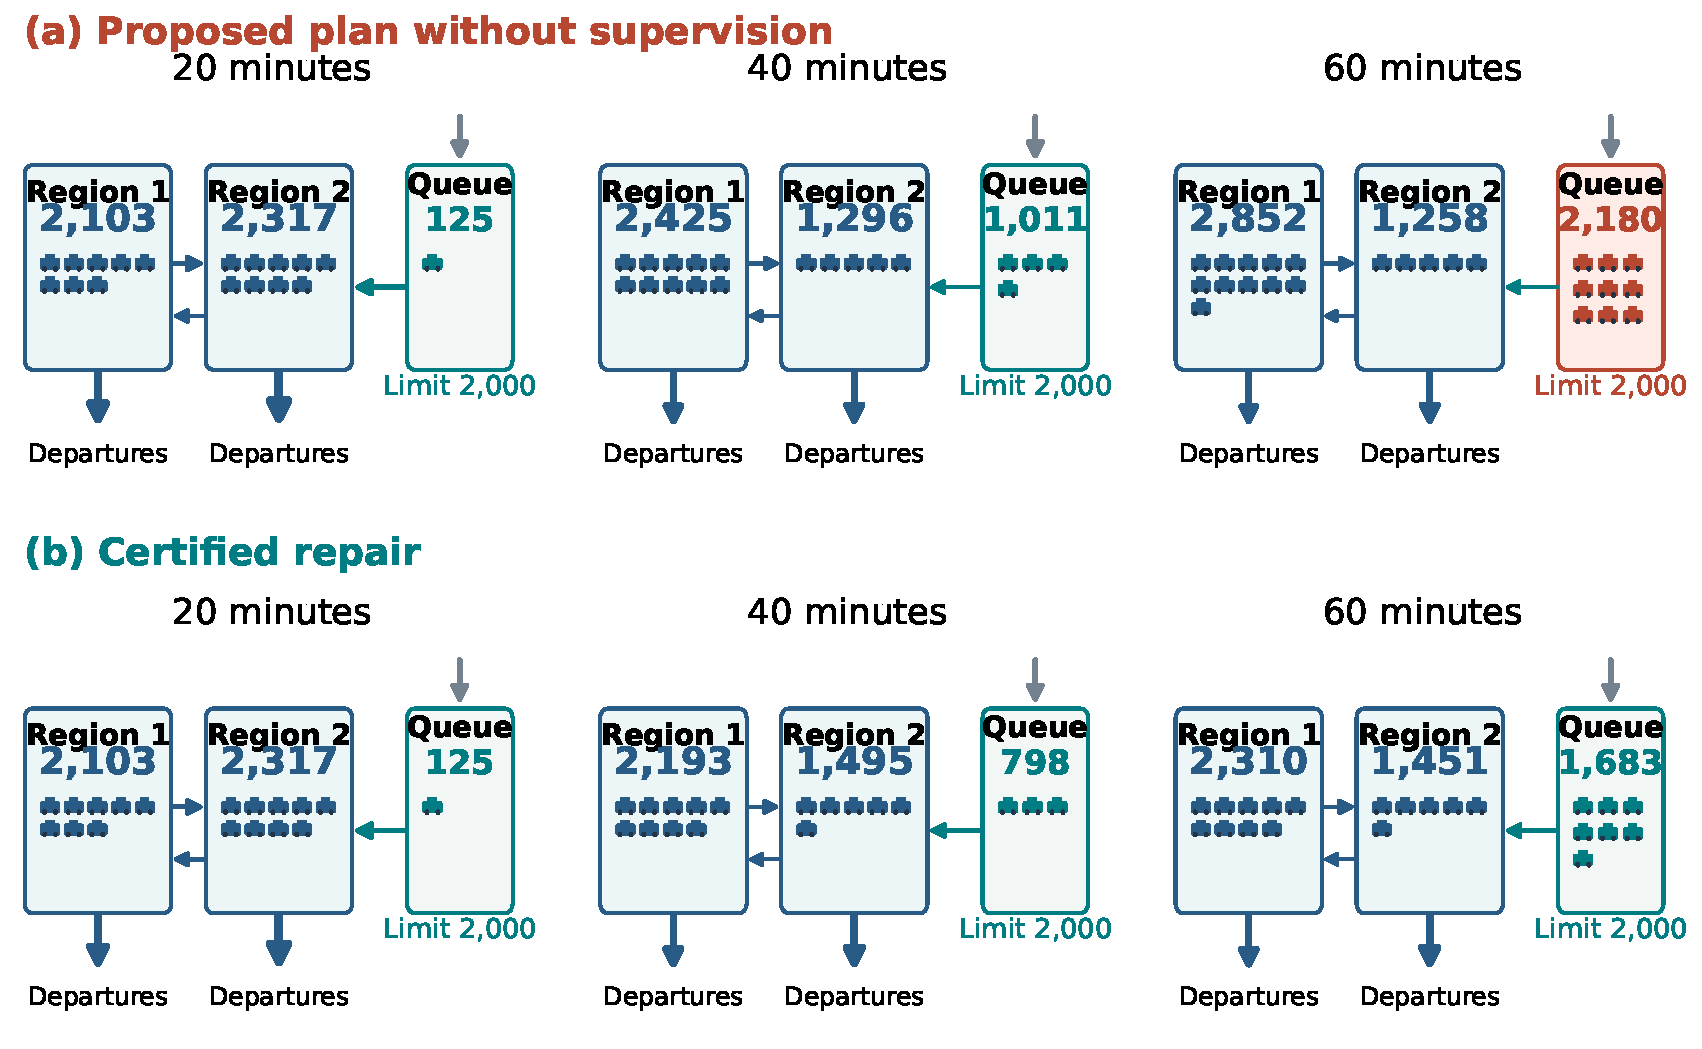
\includegraphics[width=\textwidth]{figures/supervisory_snapshots.pdf}
\caption{Traffic snapshots for the queue--deadline conflict case under the same
all-high initial state and $+300$~veh/h arrival error. Numbers are simulated
vehicle counts rounded to whole vehicles. Each car icon represents
approximately 250 vehicles, with the icon count rounded to the nearest
integer. Arrows show interregional transfers, queue admission, exterior
arrivals, and departures from the modeled network; thicker arrows indicate
larger instantaneous rates on a common scale. Departures combine local
trip completion and, for Region~2, exterior exits. Internal demand remains
in the simulation but is omitted from the drawing. Red marks a queue
above its 2000-vehicle capacity. Icon positions are illustrative.}
\label{fig:traffic-snapshots}
\end{figure}
Figure~\ref{fig:supervisory-counts}(a)--(c) shows the resulting accumulations.
Unchecked nominal MPC exceeds exterior storage by about 180 vehicles
(9\%), reaching 2180 vehicles against the 2000-vehicle limit. It also
misses the Region-1 deadline by 2.2 vehicles, ending at 2852.2 vehicles.
The supervisor instead selects a certified repair with
$\lambda_{\rm rep}=0.25$. Its peak queue is 1682.7 vehicles, and its
Region-1 deadline accumulation is 2310 vehicles. The current plan
also satisfies both limits and provides a reference for the cost of
pursuing the requested regional priority.

\begin{figure}[!t]
\centering
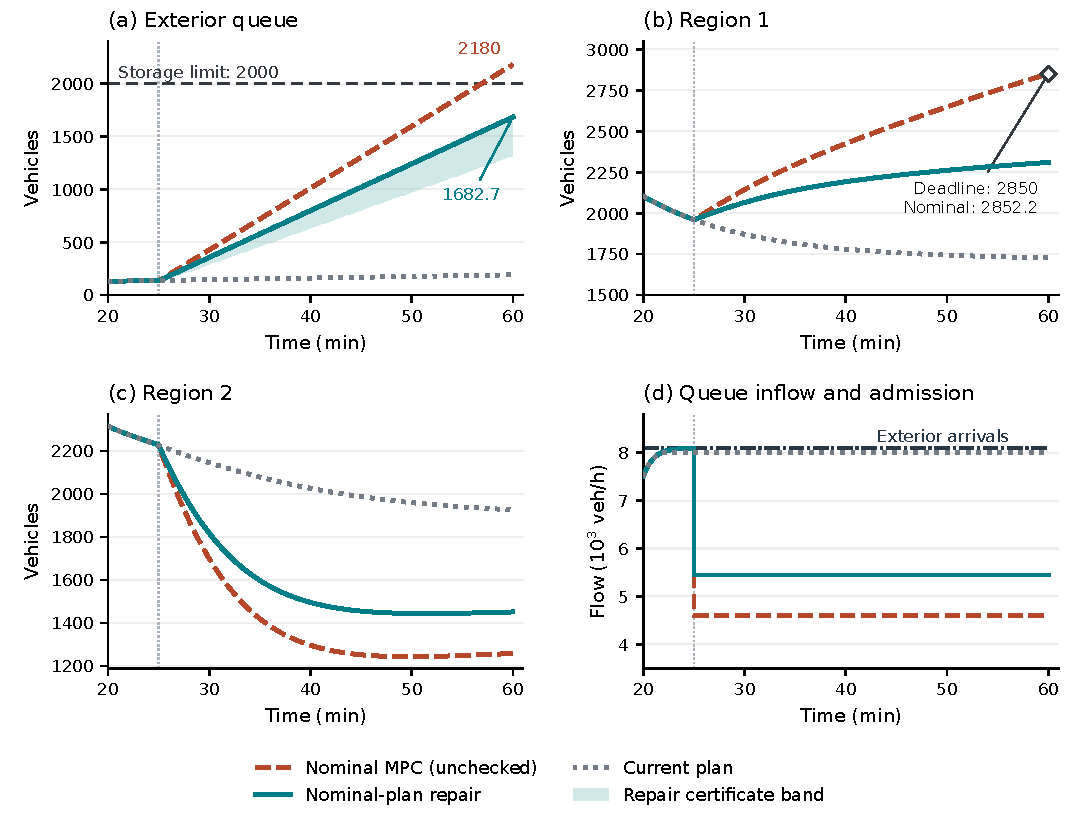
\includegraphics[width=\textwidth]{figures/supervisory_combined.pdf}
\caption{Queue--deadline conflict case with matched initial states and
arrivals: (a) exterior queue $z$, (b) Region~1 accumulation $n_1$,
(c) Region~2 accumulation $n_2$, and (d) exterior arrivals $\Lambda$ and
admission $a$ in thousands of veh/h. The dotted line marks the minute-25
input change. The horizontal line is the 2000-vehicle queue limit, and the
endpoint marker is the 2850-vehicle Region-1 requirement at minute 60.
The shaded band is the repaired plan's certified queue enclosure, whose
upper bound reaches 1682.7 vehicles.}
\label{fig:supervisory-counts}
\label{fig:supervisory-flows}
\label{fig:certified-queue-bound}
\end{figure}

The shaded enclosure covers every initial error within one vehicle
and every measurable arrival error bounded by 300~veh/h on 15-second
verification subintervals. Both the repair and current-plan certificates
cover execution through minute 60. The regional capacities of 10,000
vehicles lie above the plotted ranges.

Figure~\ref{fig:supervisory-flows}(d) explains the queue response through
the arrival and admission rates. At minute 25, the nominal plan reduces admission to
approximately 4594~veh/h, so arrivals exceed entry to Region~2 and the
exterior queue grows. Repair raises admission to approximately
5447~veh/h and increases the Region-1-to-Region-2 perimeter control input from
0.397 to 0.548. These changes reduce exterior waiting and the number of
vehicles remaining in Region~1, while allowing a higher Region-2
accumulation than the nominal proposal. The queue continues to grow under
repair, but stays within storage through the certified minute-60 expiry.
The example illustrates the finite-plan guarantees of
Proposition~\ref{prop:structure-plan} and Lemma~\ref{thm:repair-grid}.


Table~\ref{tab:benchmark-conflict} quantifies this tradeoff and includes
the other planning options on the same realization. Retention gives the
lowest TTS, while repair lowers the Region-2-weighted cost relative to
retention. The control-barrier-function quadratic program
(CBF-QP) protects storage but misses the deadline. Full-scenario MPC
satisfies both constraints on this realization, although the certification check
for the full uncertainty family is inconclusive. Thus the table distinguishes the
observed traffic performance from the guarantee available for execution.
For the same realization, completed trips are 15,924 for nominal MPC,
16,770 for repair, and 18,365 for retention, rounded to whole vehicles.
These counts agree with the total-accumulation balance in
\eqref{eq:new-conservation} and help explain the lower TTS under retention.
The plotted trajectories use the stored control inputs and were checked by
independent adaptive integration against the original simulations and the
regional and queue conservation balances.

\begin{table}[!htbp]
\centering\footnotesize
\setlength{\belowcaptionskip}{6pt}
\caption{Matched adverse realization, minutes 20--60. TTS is total time
spent and $J_D$ is the Region-2-weighted cost ($p=4$), both in veh-h.
Peak queue and deadline accumulation $n_1(E)$ are in vehicles, with limits
2000 and 2850. P/S gives physical/service outcomes (P: pass, F: fail).
Cert. gives full-family certification (Yes: certified, No: inconclusive,
or a demonstrated violation; dash: not assessed). MPC is model predictive
control and CBF-QP is a control-barrier-function quadratic program.
Values are rounded to whole units except the repaired peak queue.}
\label{tab:benchmark-conflict}
\setlength{\tabcolsep}{3pt}
\begin{tabular}{@{}lrrrrcc@{}}
\toprule
Policy & TTS & $J_D$ & Peak queue & $n_1(E)$ & P/S & Cert.\\
\midrule
Nominal MPC & 3300 & 6328 & 2180 & 2852 & F/F & No\\
CBF-QP & 3295 & 6376 & 1844 & 2917 & P/F & ---\\
Current plan & 2695 & 6814 & 194 & 1727 & P/P & Yes\\
Nominal-plan repair & 3097 & 6427 & 1682.7 & 2310 & P/P & Yes\\
Full-scenario MPC & 3267 & 6357 & 1999 & 2848 & P/P & No\\
Full-scenario repair & 3075 & 6453 & 1547 & 2314 & P/P & Yes\\
\bottomrule
\end{tabular}
\end{table}

The certificate band in Figure~\ref{fig:certified-queue-bound}(a)
leaves at least 317.3 vehicles of storage throughout the repair.



\subsection{Recovery from congested conditions}
\label{sec:congested-results}

We next test whether the same certification and repair procedure can
support recovery when both regions begin on the decreasing branch of
the MFD. The estimated initial state is
$(4500,4500,2250,2250,750,750,500)$ vehicles in the order of $x$.
Both regional totals exceed the critical accumulation of 3391.93 vehicles,
and the initial destination shares match those of the reference state.
The MFD, internal demands, admission law, input bounds, and physical
capacities remain unchanged. Exterior arrivals rise from 6000 to
7800~veh/h between minutes 15 and 20 and remain at that level through
minute 60. Plans have constant inputs over minutes 0--5 and 5--60.
The service requirement limits Region~1 to 3300 vehicles at minute 60,
written $n_1(1)\le3300$ because model time is measured in hours.

The proposed plan minimizes the nominal Region-2-weighted cost with
$p=4$. A backup candidate is prepared using a balanced objective, an
upper-state planning scenario with component increments
$(25,25,25,25,25,25,10)$ vehicles and an arrival rate 300~veh/h above
the forecast, and planning clearances
of 1600 vehicles for the queue and 3000 vehicles for the deadline.
These clearances guide the numerical planning tool. The independent
certification check retains the 2000-vehicle physical queue limit and
3300-vehicle service limit. Planning and certification are completed
before execution in this experiment.

The primary uncertainty set is
$d_x=(25,25,25,25,25,25,10)^\top$ vehicles with
$\bar w=300$~veh/h. Certification uses destination-specific coordinates and a four-box
subdivision of the initial uncertainty set. The subdivision bisects the $n_1$ and $n_2$
intervals at their estimated values, leaving every other interval unchanged.
All four boxes must pass. Verification uses signed generators, independently
verified nonnegativity and queue bounds, and 15-second verification intervals.
The complete backup and repaired-plan certificates verify capacity-limited
admission on every interval. No regional independence from arrival error
is assumed before those branch checks.

The backup passes all four checks. On the interpolation grid with spacing
0.05, repair first succeeds at $\lambda_{\rm rep}=0.35$. Every preceding
grid candidate admits an allowed queue overflow. Indeed, $a\le\kappa_{02}u_{02}$
gives the exact balance bound
\[
 z(1)\ge z(0)+\int_0^1\Lambda(t)\,dt
                  -\kappa_{02}\int_0^1u_{02}(t)\,dt.
\]
For the upper initial queue and constant arrival error $+300$~veh/h,
exact arithmetic with the implemented coefficients makes this lower bound
exceed 2000 vehicles for each earlier grid weight, including the proposal.
Thus rejection is supported by a violating allowed condition. The first
passing weight is a result for this finite compiled grid.

\begin{figure}[!t]
\centering
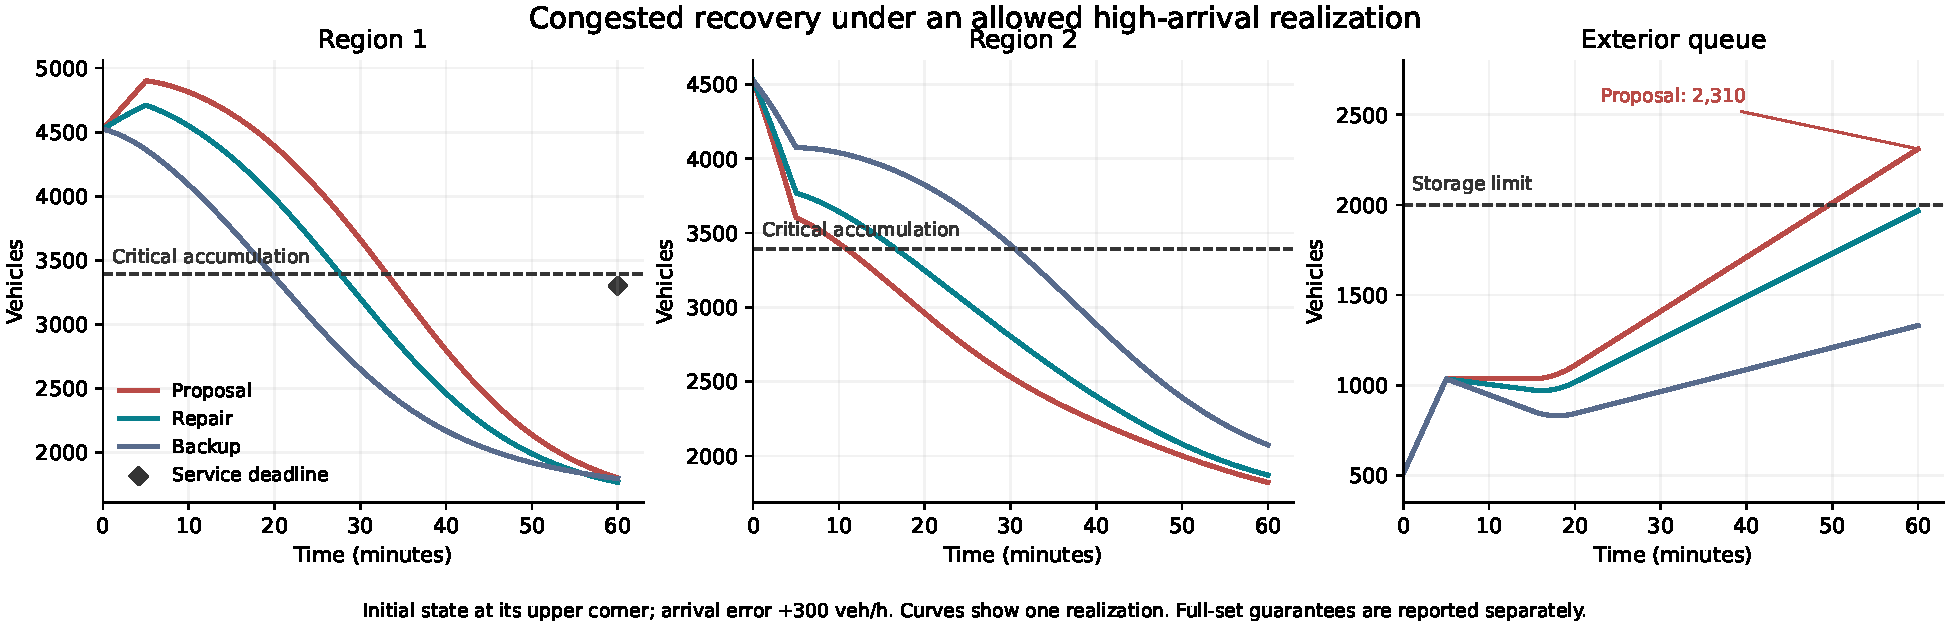
\includegraphics[width=\textwidth]{figures/wide_uncertainty_recovery.pdf}
\caption{Congested recovery for the proposed plan, the certified repair and
the certified backup. The displayed realization uses the upper initial
state corner and arrival error $+300$~veh/h. Dashed lines mark the
3391.93-vehicle critical accumulation and the 2000-vehicle queue capacity;
the diamond marks $n_1(1)\le3300$. Curves are simulated realizations,
while the guarantees in the text cover the full uncertainty family.
The proposed trajectory continues after overflow to show the consequence
of unchecked execution; spatial spillback is not modeled.}
\label{fig:congested-counts}
\end{figure}

The repaired plan guarantees a continuous queue maximum below 1968 vehicles
and minute-60 upper bounds of 2119 vehicles in Region~1 and 2320 in
Region~2, rounded upward.
The backup gives corresponding bounds of 1331, 2170 and 2675 vehicles.
Both regions therefore finish below the critical accumulation for every
allowed initial state and measurable arrival error. The Region-1 service
requirement has substantial slack: its repaired bound is 2119 against 3300.
This case establishes storage protection and recovery with that deadline,
while the separate deadline studies examine tighter service requirements.

\begin{table}[!htbp]
\centering\small
\caption{Congested-start comparison over 60 minutes with regional state
error bounds of 25 vehicles, queue error 10 vehicles and arrival error
300~veh/h. Maximum queue is the largest value in 640 matched simulations;
physical and service passes count simulations satisfying those constraints.
TTS is total time spent in both regions and the queue. $J_D$ is the
Region-2-weighted cost with $p=4$; both costs are medians in vehicle-hours.
Certificates cover the full uncertainty family.}
\label{tab:congested-results}
\begin{tabularx}{\linewidth}{@{}Xrrr@{}}
\toprule
Measure & Proposed & Repaired & Backup\\
\midrule
Maximum simulated queue (vehicles) & 2310.0 & 1967.2 & 1330.7\\
Physical passes & 320/640 & 640/640 & 640/640\\
Service passes & 640/640 & 640/640 & 640/640\\
Median TTS (vehicle-hours) & 7488.3 & 7229.7 & 7011.1\\
Median $J_D$ (vehicle-hours) & 15499.7 & 15773.9 & 16789.5\\
Full-hour certificate & Rejected & Passed & Passed\\
\bottomrule
\end{tabularx}
\end{table}

Relative to the backup, repair reduces median priority cost by 6.05\%
with 3.12\% greater median TTS, preserving 78.74\% of the proposal's
priority-cost improvement. These are matched-simulation performance
statistics. Two-second Runge--Kutta evaluations and independent adaptive
DOP853 trajectories agree within 0.1 vehicles or vehicle-hours for the
stored adverse realization.

\begin{figure}[!t]
\centering
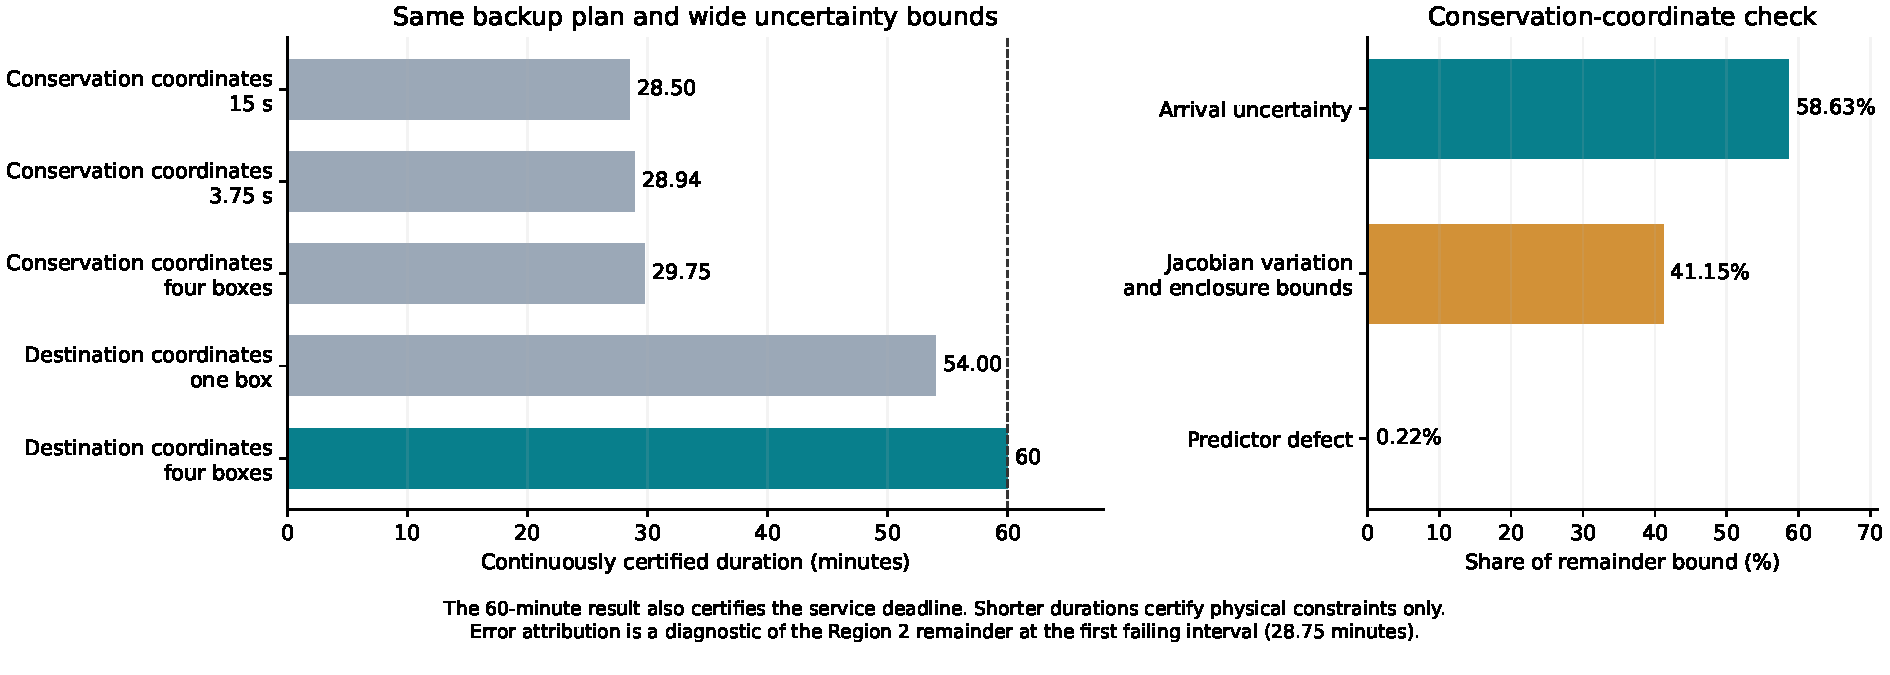
\includegraphics[width=\textwidth]{figures/certification_diagnostics.pdf}
\caption{Verification diagnostics for the unchanged congested backup and
the wider uncertainty set. Left: continuous physical-constraint prefixes
certified by each configuration; the 60-minute result also certifies the
service deadline. Shorter prefixes do not certify that deadline or a
replanning period. Right: diagnostic attribution of the Region-2 remainder
bound at the first failing original interval, ending at 28.75 minutes.
The shares use the computed comparison matrices and are not independent
certificates or physical error measurements.}
\label{fig:congested-diagnostics}
\end{figure}

The original conservation-coordinate check reaches 28.5 minutes. Reducing
the verification step from 15 to 3.75 seconds reaches 28.94 minutes, and splitting
alone reaches 29.75. Destination-specific coordinates reach 54 minutes;
combining them with the subdivision certifies the full hour. The original
failing remainder is dominated by propagated arrival forcing (58.63\%)
and Jacobian/generator mismatch (41.15\%), with 0.22\% attributed to the
predictor defect. This supports improving uncertainty propagation for this
case. It does not establish that predictor accuracy is negligible in other
operating regimes.

Residual regional conservatism remains substantial. The backup's certified
terminal widths for $n_1,n_2$ are approximately 745 and 1207 vehicles,
compared with sampled spreads of 28 and 67. For repair they are 691 and
893, compared with 58 and 42. These ratios range from about 12 to 27;
passing certificates benefit from the available constraint margins.
The queue's certified and sampled terminal widths both equal 620 vehicles
to numerical precision: 20 vehicles of initial spread plus
$2(300)(1)=600$ vehicles from arrival error. The samples do not establish
the full regional reachable sets. The 25-vehicle regional error is about
0.56\% of the initial 4500 vehicles, so field estimation accuracy remains
an open deployment requirement.

The smaller one-vehicle, 60~veh/h case and all unsuccessful diagnostic
checks are retained in the repository. The fixed-portfolio timings below include unsuccessful configurations
and every attempted sub-box. Detailed budgets and horizon sweeps are
supplied with the reproduction records.

\paragraph{Starting accumulation and verification time}
At 4500 vehicles the fitted outflow is 7.05\% below its peak. To examine
how far the same plans extend, we increase the initial total in both
regions over $\{3500,4000,4500,5000,5500,6000,6500,7000,8000,9000\}$
vehicles. Destination proportions, the 500-vehicle initial queue, uncertainty
bounds, forecasts, control schedules and minute-60 deadline are fixed.
Each plan uses the same ordered portfolio. A configuration uses signed
propagation on either the whole box or its four outward-rounded sub-boxes;
subdivision stops after a failed component, and the portfolio stops after
a complete pass. This tests the stored plans rather than replanning for
each starting accumulation.

\begin{table}[!htbp]
\centering\small
\caption{Fixed-plan congestion sweep. Both plans start from the same
estimated accumulation $n_1=n_2$. D1 denotes a complete certificate in
unsplit destination coordinates, and D4 denotes one obtained from all
four destination-coordinate sub-boxes. A dash means no portfolio member
certifies the full physical and service contract. Every passing case
also places both regional terminal upper bounds below critical accumulation.
These are tested grid values, not an exact recovery boundary.}
\label{tab:congestion-depth}
\begin{tabular}{@{}rcc@{}}
\toprule
Initial vehicles per region & Backup & Repaired plan\\
\midrule
3500 & D1 & D1\\
4000 & D1 & D1\\
4500 & D4 & D4\\
5000, 5500, 6000 & --- & ---\\
6500, 7000, 8000, 9000 & --- & ---\\
\bottomrule
\end{tabular}
\end{table}

Thus 4500 vehicles is the largest tested starting accumulation with
certified recovery for these fixed plans. At 5000 vehicles, an allowed
upper-corner, high-arrival simulation leaves the backup's Region~2 at
3520 vehicles, above critical accumulation, while the repaired plan
ends with 6596 vehicles in Region~1 and misses its 3300-vehicle deadline.
Higher-start simulations also encounter regional storage violations.
Trajectories beyond the first storage violation are excluded from physical
interpretation. The unsuccessful certificates do not establish that no
other plan can recover from those initial conditions.

At the 4500-vehicle setting, the portfolio checks six initial sets per
plan: the two unsplit configurations and all four destination-coordinate
sub-boxes. Total measured verification time is 82.6 seconds for the backup
and 82.3 seconds for repair, including the unsuccessful checks. The times
are measured on an Intel Core Ultra 7 255H with six worker processes
checking different cases; configurations and sub-boxes within each case
run sequentially. They exclude planning, sensing and actuation and are
not worst-case response-time guarantees. Planning and checking occur
before execution in this experiment.

\subsection{Effect of traffic structure on certification}
\label{sec:structure-results}
\label{sec:structure-online}

To identify the contribution of traffic structure, this study changes the state-bound
construction while holding the proposed plan and information fixed.
Figure~\ref{fig:structure-comparison} shows both the resulting deadline
bounds and whether every physical and service check passes.
\begin{figure}[!t]
\centering
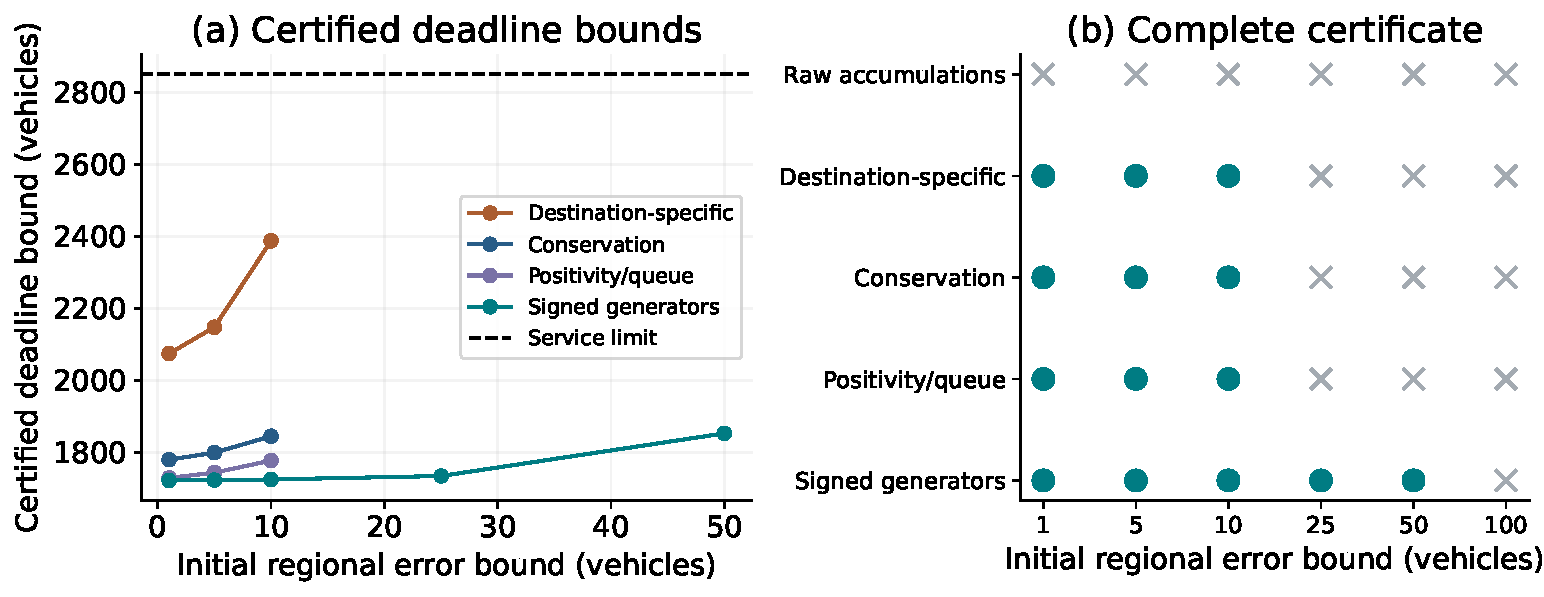
\includegraphics[width=\textwidth]{figures/structure_certification_comparison.pdf}
\caption{Effect of traffic structure for the fixed-plan experiment.
(a) Region-1 deadline bounds for complete passing certificates, with
the 2850-vehicle service limit marked. Lines connect tested settings only.
(b) Every tested initial regional error bound: circles indicate a complete
certificate and crosses an inconclusive check. Queue uncertainty is
capped at 10 vehicles, and the arrival-error bound is 60~veh/h.
No deadline value is plotted when an earlier physical check prevents
completion. Destination-specific denotes coordinates for the separate
destination accumulations; conservation adds their allocated queue shares.}
\label{fig:structure-comparison}
\end{figure}

The largest tested certifiable regional half-width is 50 vehicles with
signed propagation, compared with 10 vehicles for the interval methods,
at a 60~veh/h arrival-error bound. To separate the coordinate effect
from the propagation method, Table~\ref{tab:coordinate-comparison} compares
five representations for the same fixed two-block MPC plan, forecast,
initial state, and 15-second verification partition. All methods test
$d\in\{1,5,10,25,50,100\}$ with
$d_x=(d,d,d,d,d,d,\min(d,10))^\top$ vehicles and a 2850-vehicle
Region-1 deadline limit. Destination-specific coordinates
give a 2075-vehicle deadline bound at $d=1$. Including the queue shares
reduces it to 1780 vehicles. Both representations pass through $d=10$ on
the tested grid, while checks using raw accumulation boxes remain inconclusive throughout
that grid.

\begin{table}[!htbp]
\centering\small
\setlength{\belowcaptionskip}{6pt}
\caption{Fixed-plan certification over minutes 0--60. Bounds on the
Region-1 deadline accumulation are rounded upward to whole vehicles.
The largest passing initial error $d$ is a tested grid value; None means
no complete certificate passes. The last column identifies the first
check not certified at the first nonpassing tested $d$. This is not an
observed traffic violation.}
\label{tab:coordinate-comparison}
\setlength{\tabcolsep}{3pt}
\footnotesize
\begin{tabularx}{\linewidth}{@{}Xrrr>{\raggedright\arraybackslash}p{0.29\linewidth}@{}}
\toprule
Representation & \shortstack{Bound at\\$d=1$} & \shortstack{Largest\\passing $d$} & \shortstack{Bound at\\largest $d$} & \shortstack[l]{First check\\not certified}\\
\midrule
Raw accumulations & --- & None & --- & $n_{12}\ge0$ at $d=1$\\
Destination-specific accumulations & 2075 & 10 & 2388 & $n_{20}\ge0$ at $d=25$\\
Conservation coordinates & 1780 & 10 & 1845 & $n_{20}\ge0$ at $d=25$\\
Positivity/queue & 1729 & 10 & 1777 & $n_2\le10{,}000$ at $d=25$\\
Signed generators & 1722 & 50 & 1853 & $n_2\le10{,}000$ at $d=100$\\
Fixed portfolio & 1722 & 50 & 1853 & No complete pass at $d=100$\\
\bottomrule
\end{tabularx}
\end{table}

The fixed portfolio passes at $d=1,5,10,25,50$ through its first,
conservation-coordinate signed configuration. No member passes at $d=100$,
so the largest tested passing uncertainty is unchanged.

The queue-capped uncertainty in Table~\ref{tab:coordinate-comparison}
differs from the equal seven-state half-widths used for minute-20
replacement. In particular, the 50-vehicle result retains a 10-vehicle
queue half-width. Thus this result describes the specified uncertainty
set, not a general maximum estimation error tolerated by the framework. At a larger 300~veh/h arrival-error bound and $d=1$,
positivity/queue propagation gives a tighter deadline bound than signed
propagation (2009 versus 2256 vehicles). At $d=25$, only the signed
method passes, with a 2504-vehicle bound. The refinements therefore give
complementary checks, and acceptance requires every constraint to pass.

The first nonpassing checks in Table~\ref{tab:coordinate-comparison}
concern nonnegativity or regional capacity. Their failure shows that the
computed enclosure is insufficient to certify the plan, without proving
that a trajectory violates a constraint. A separate service-margin
comparison is reported in \appref{app:additional-numerics}.

The advantage of conservation coordinates in this fixed-plan comparison
is specific to its dynamics and uncertainty sets. The capacity-limited
congested case shows the opposite coordinate ordering. Together these
studies support matching coordinates to verified traffic structure,
rather than a universal superiority claim for conservation coordinates.

\subsection{Performance across operating conditions}

\label{sec:uncertainty-results}

We now move from individual plans to a broader set of operating
conditions. The questions are how often the tools provide a certified
plan, how much repair increases that availability, and what traffic cost
is associated with retaining the requested regional priority.
The broader regional-priority comparison returns to the common minute-20 state and
the 30\% one-hour event. Its 72 development contracts cross initial-state
half-widths $d\in\{1,10,25,50\}$ vehicles, arrival-error bounds
$\bar w\in\{60,150,300\}$ veh/h, deadline limits
$\eta\in\{2750,2850,2950\}$ vehicles, and Region-2 weights $p\in\{2,4\}$.
Eight held-out contracts use $d\in\{5,20\}$,
$\bar w\in\{100,225\}$, $\eta\in\{2800,2900\}$, and $p=3$.
Full-scenario MPC constrains the 640 scenarios and the center forecast
with one-vehicle prediction clearance. Its settings are fixed across the development and held-out sets,
without case-specific retuning; the reproduction records describe their
selection using development cases. The held-out contracts test intermediate parameter values.
Here $d_x=d\mathbf1_7$ throughout, including the queue. Nine nominal
plans pass at $d=50$ vehicles without a separate queue cap.

\begin{table}[!htbp]
\centering\small
\setlength{\belowcaptionskip}{6pt}
\caption{Regional-priority baseline study with 80 contracts, using the unsplit
conservation-coordinate signed certification procedure. Candidate simulation
passes require all 640 realizations in a contract to pass. Certified
availability counts contracts with a passing plan, while the final column
tests only the outputs actually selected by the checked procedure.
MPC is model predictive control. A dash identifies a candidate-only
comparison or a procedure reported through its selected outputs.}
\label{tab:benchmark-deadlines}
\footnotesize
\setlength{\tabcolsep}{4pt}
\begin{tabularx}{\linewidth}{@{}Xrrr@{}}
\toprule
Planning/execution option & \shortstack{Candidate\\simulation\\passes} &
\shortstack{Certified\\output\\available} &
\shortstack{Simulation passes\\among selected\\outputs}\\
\midrule
Nominal MPC & 36/80 & 36/80 & ---\\
Five-scenario MPC & 40/80 & 40/80 & ---\\
Full-scenario MPC & 80/80 & 44/80 & ---\\
\midrule
Nominal MPC with checked repair & --- & 74/80 & 74/74\\
Full-scenario MPC with checked repair & --- & 74/80 & 74/74\\
Repair with a newly certified backup & --- & 80/80 & 80/80\\
\bottomrule
\end{tabularx}
\end{table}

Table~\ref{tab:benchmark-deadlines} shows that full-scenario MPC passes
all tested simulations in every contract, while certification over the full
uncertainty family succeeds in 44/80 with the baseline procedure. Checking the remaining current plan against the new
contract establishes a certified backup in 68/80. The conservation-coordinate procedure
selects 36 nominal proposals and 38 repairs, giving 74 certified outputs.
No certified output is selected under the new contract in the other six
cases. The simulations of an uncertified current-plan comparator in those
cases are not executions authorized by this procedure. A previous
certificate can still apply under its original conditions, as explained
in Section~\ref{sec:supervisory-agent}.

Newly constructed backups pass in all twelve contracts where the current
plan does not pass the new check. Six already have certified nominal
proposals, while the other six gain a certified output, raising availability
to 80/80. This illustrates the same-contract backup requirement in
Lemma~\ref{thm:repair-grid}. The breakdown by initial-state and arrival-error
bounds is in Table~\ref{tab:availability-breakdown}.
Separately, the CBF-QP satisfies physical constraints in all
80 adverse runs and the deadline in 44, using one adverse realization per
contract. Its instantaneous physical barriers and the scheduled service
requirement therefore lead to different outcomes.

Across the 80 contracts, nominal MPC violates queue storage in 44
contracts and the service deadline in 36. Taking the largest observed
excess within each affected contract, queue overflow ranges from 36.0 to
242.7 vehicles, with median 90.3. Deadline excess ranges from 1.3 to
65.4 vehicles, with median 19.4. These are simulation-based violation sizes,
reported separately from inconclusive certification outcomes.

To quantify the traffic cost of repair, compare nominal, current, and
repaired plans $P^0,P^B,P^R$ on a common realization $\omega=(x_0,w)$.
Here $P^R$ is the repaired plan selected for execution, and
$J_Q(P;\omega)$ and $J_D(P;\omega)$ abbreviate the corresponding costs
with initial state $x_0$ and arrival error $w$. The priority
improvement $\Delta J_\omega$, change in TTS
$\Delta D_\omega$, and recovered requested benefit $B_\omega$ are
\begin{equation}
\begin{aligned}
\Delta J_\omega&=100\frac{J_D(P^B;\omega)-J_D(P^R;\omega)}{J_D(P^B;\omega)},\\
\Delta D_\omega&=100\frac{J_Q(P^R;\omega)-J_Q(P^B;\omega)}{J_Q(P^B;\omega)},\\
B_\omega&=\frac{J_D(P^B;\omega)-J_D(P^R;\omega)}{J_D(P^B;\omega)-J_D(P^0;\omega)}.
\end{aligned}
\label{eq:benchmark-repair-metrics}
\end{equation}
Positive $\Delta J_\omega$ means that repair improves the priority
objective relative to retention, while positive $\Delta D_\omega$ means
that it increases TTS. These changes and $100B_\omega$ are percentages.
Across 24,320 matched realizations from the 38 contracts repaired using
the current-plan backup, every denominator in $B_\omega$ is positive.
Median priority improvement relative to the current plan is 5.7\%
(interquartile range 3.9--6.2\%), median TTS increase is 16.1\%
(8.8--19.6\%), and median recovered requested benefit is 91.7\%
(78.2--95.9\%). Figure~\ref{fig:repair-distribution} displays these distributions.
The ranges describe the middle half of the pooled matched realizations,
not confidence intervals. Repair therefore recovers much of
the requested regional preference in these cases, with a measured increase
in TTS. These realized costs complement the analytical
bound in Proposition~\ref{prop:repair-cost}, which requires its stated
common-domain and regularity assumptions.


\begin{figure}[!t]
\centering
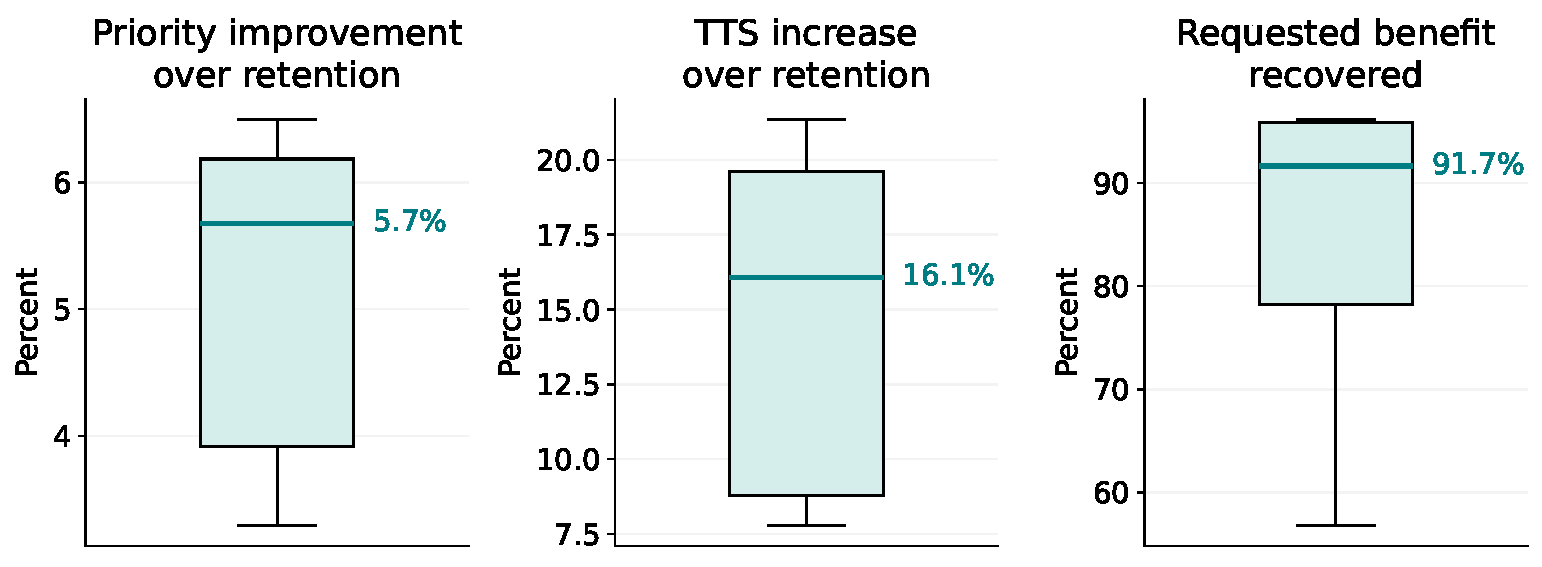
\includegraphics[width=\textwidth]{figures/repair_cost_distribution.pdf}
\caption{Traffic consequences of repair over 24,320 matched realizations
from 38 contracts. The panels show priority improvement over retention,
TTS increase over retention, and the fraction of the requested priority
benefit recovered, all expressed as percentages using
\eqref{eq:benchmark-repair-metrics}. Boxes span the 25th--75th percentiles,
central lines mark medians, and whiskers mark the 5th--95th percentiles.
The nominal proposal defines the requested benefit even when it cannot
be executed. The distributions pool specified test realizations and are
not confidence intervals.}
\label{fig:repair-distribution}
\end{figure}
\paragraph{Fixed-portfolio verification of the stored proposals}
The same portfolio rechecks all 80 nominal and 80 full-scenario proposals
under their original contracts. It certifies 36 nominal proposals and
50 full-scenario proposals, compared with 36 and 44 under the single
conservation-coordinate signed check. All earlier passes are retained.
The six additional full-scenario passes use unsplit destination coordinates;
subdivision adds no further passes in this comparison. The six added
certificates are in the development set; the held-out outcomes are unchanged.
These results measure the verification rule on fixed plans. The repair
searches and performance comparisons above are separate baseline results.

\begin{table}[!htbp]
\centering\small
\caption{One fixed verification portfolio applied to 160 stored proposals.
C1 and D1 denote unsplit conservation and destination coordinates.
No additional proposal passes through a four-box member. Times are total
elapsed verification time per proposal, including every unsuccessful
configuration and attempted sub-box, measured under the same six-worker
conditions as the congestion sweep. Planning time is excluded.}
\label{tab:fixed-portfolio}
\begin{tabularx}{\linewidth}{@{}Xrr@{}}
\toprule
Measure & Nominal MPC & Full-scenario MPC\\
\midrule
Passing proposals & 36/80 & 50/80\\
First passing member C1 & 36 & 44\\
First passing member D1 & 0 & 6\\
No complete certificate & 44 & 30\\
Median time (s) & 40.1 & 10.7\\
Observed time range (s) & 9.3--89.7 & 9.7--72.7\\
\bottomrule
\end{tabularx}
\end{table}

The extra configurations improve availability for some full-scenario
plans and increase computation for inconclusive cases. Acceptance still
requires a complete matching certificate before activation. The recorded
timings do not establish that a proposal can always be checked within a
given decision interval.

\subsection{Successive requests and computation delays}
\label{sec:sequential-handover-results}

The preceding studies evaluate a decision from a specified initial set.
During repeated operation, each new request instead inherits the traffic
state produced by earlier decisions. We first examine replacements at
fixed activation times, then allow time for planning and certification.
The service deadline remains at minute 60 throughout both studies.

\paragraph{Successive plan requests}
A certified regional-priority repair with Region-2 weight $p=4$ starts at minute 20.
At minute 25, a request proposes the remaining $p=2$ full-scenario plan,
and at minute 30 another request proposes the remaining $p=4$ nominal
plan. These are stored planner outputs, used to isolate the supervisory
decision from language interpretation. Physical constraints and uncertainty
bounds remain fixed. Each replacement is checked from a box containing
the states reachable under the active plan. Rejection preserves that
plan's original schedule, stored certificate, and expiry, as required by
Theorem~\ref{thm:new-plan-closure}.

\begin{table}[!htbp]
\centering\small
\setlength{\belowcaptionskip}{6pt}
\caption{Successive regional-priority requests. The decision column lists
the minute-25 and minute-30 outcomes. Feasible simulations satisfy the
physical and service requirements out of 640 matched realizations.
TTS is total time spent in veh-h over minutes 20--60. Current keeps the
initial plan, Unchecked executes both replacements, and Supervised
executes only certified replacements.}
\label{tab:sequential-handover}
\footnotesize
\setlength{\tabcolsep}{3pt}
\begin{tabularx}{\linewidth}{@{}>{\raggedright\arraybackslash}Xcccccc@{}}
\toprule
Case & \shortstack{Decisions\\25/30 min} & \multicolumn{2}{c}{Feasible simulations} & \multicolumn{3}{c}{Median TTS (veh-h)}\\
 & & Unchecked & Supervised & Current & Unchecked & Supervised\\
\midrule
Low arrival error & \shortstack{Accept/\\Accept} & 640/640 & 640/640 & 3196 & 3081 & 3081\\
Queue--deadline conflict & \shortstack{Accept/\\Retain} & 640/640 & 640/640 & 3037 & 3081 & 2717\\
Wide initial uncertainty & \shortstack{Retain/\\Retain} & 640/640 & 640/640 & 3169 & 3094 & 3169\\
Tight deadline & \shortstack{Accept/\\Retain} & 512/640 & 640/640 & 2963 & 3070 & 2719\\
\bottomrule
\end{tabularx}
\end{table}

Table~\ref{tab:sequential-handover} covers acceptance of both requests,
acceptance followed by retention, and retention at both decisions.
For the low-arrival-error, queue--deadline conflict, wide-initial-uncertainty,
and tight-deadline cases, the triples
$(d,\bar w,\eta)$ are $(1,60,2850)$, $(1,300,2850)$,
$(50,60,2950)$, and $(1,300,2750)$, respectively, in vehicles, veh/h,
and vehicles. The first three cases were preselected. The tight-deadline
case is the first overflow found in the complete comparison of matched
priority weights. In the queue--deadline conflict case, the service check for
the second request is inconclusive even though its sampled unchecked schedule satisfies the
constraints. In the wide-initial-uncertainty case, the propagated boxes include inadmissible states,
without establishing that an actual trajectory reaches them. These cases
show why an inconclusive certification check must be distinguished from a
demonstrated violation.

Figure~\ref{fig:successive-traffic} shows how these decisions affect the
queue and Region~1 in the tight-deadline case. The supervisor accepts the
first replacement and retains it after rejecting the second request,
so the traffic trajectory reflects both decisions.

\begin{figure}[!t]
\centering
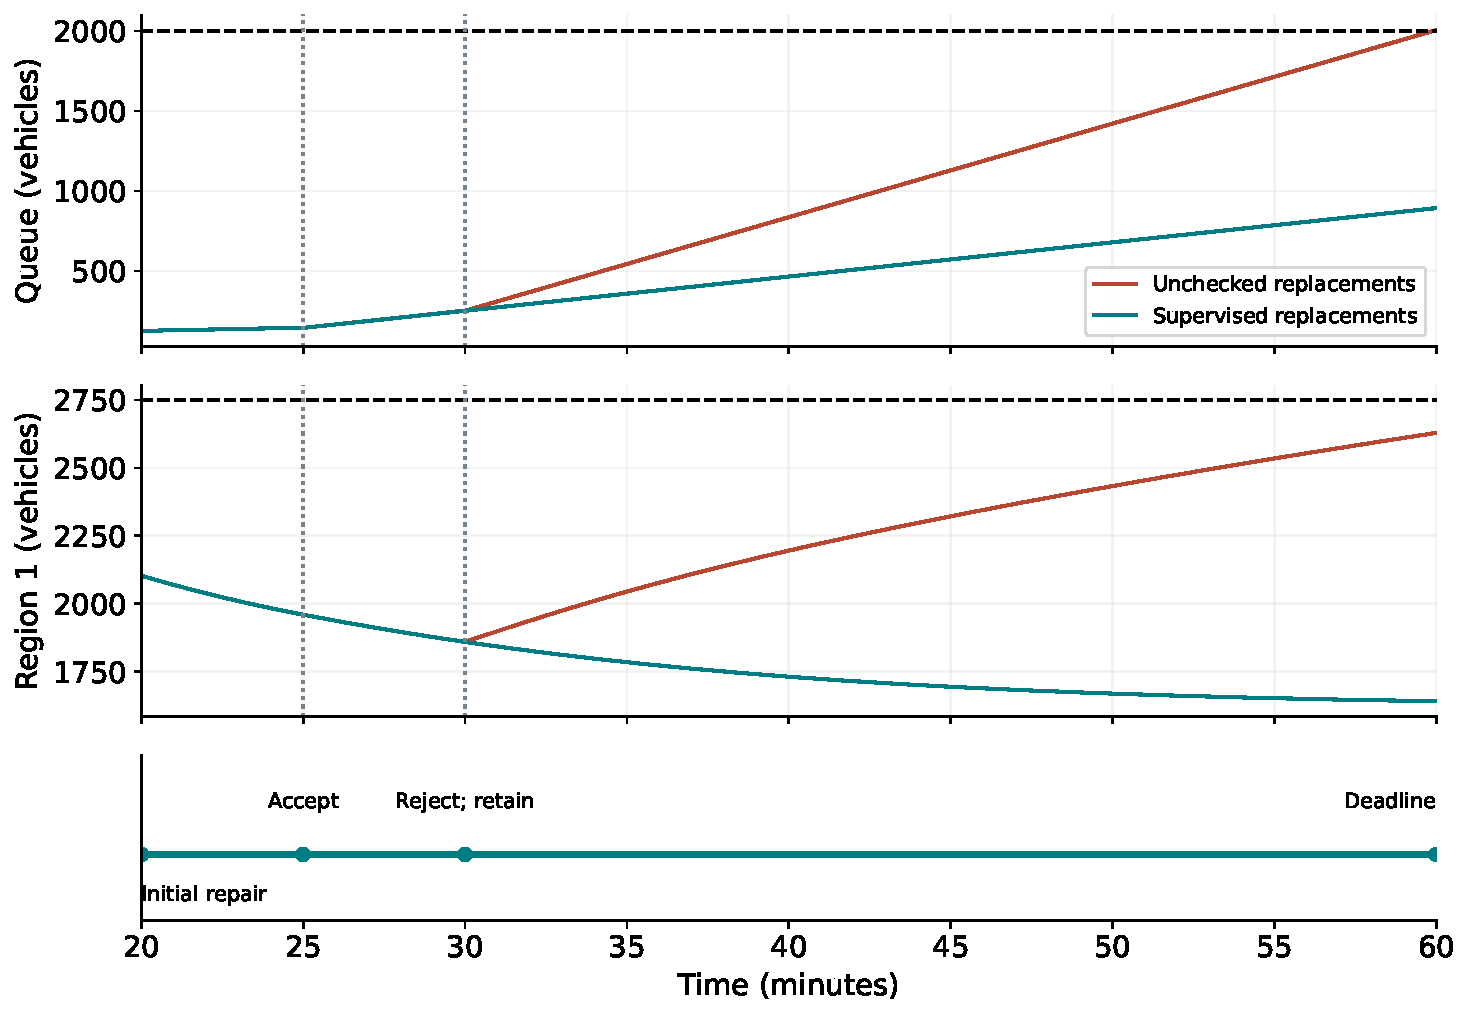
\includegraphics[width=\textwidth]{figures/successive_decisions_traffic.pdf}
\caption{Successive requests in the tight-deadline case, with the same
all-high initial corner and constant $+300$~veh/h arrival error for both
executions. The upper panels show exterior waiting and Region-1
accumulation. Dashed horizontal lines mark the 2000-vehicle queue
capacity and 2750-vehicle service limit at minute 60. Vertical dotted
lines identify requests at minutes 25 and 30. The lower timeline gives
the supervisory decisions. The unchecked schedule activates both
proposals; the supervised schedule retains the minute-25 replacement
after rejecting the minute-30 proposal.}
\label{fig:successive-traffic}
\end{figure}
The development scan pairs the $p=2$ and $p=4$ plans under each of
36 otherwise identical contracts. Thirty pairs have the certified plans
needed to initialize and test the sequence. Unchecked switching
overfills storage in three of these 30 cases, all subsequently tested by
the sequential certification procedure. In the tight-deadline case in Table~\ref{tab:sequential-handover},
the minute-25 replacement passes,
but the minute-30 request fails the queue check. Executing both requests
unchecked reaches 2005.59 vehicles against the 2000-vehicle limit,
confirmed by independent adaptive integration. Retaining the current
plan gives 640/640 physically and service-feasible simulations. Its median
TTS is 8.2\% below retaining the initial plan, while its median
cost evaluated with the requested priority weight at each time is
5.2\% above unchecked switching. The three violating pairs have maximum queue excesses of 5.59, 9.62,
and 17.60 vehicles, respectively, against the 2000-vehicle capacity.


\paragraph{Planning and checking before activation}
\label{sec:delayed-handover-results}
The delay study tests Proposition~\ref{prop:planned-handover} using
seventeen contracts with one-, two-, and five-minute activation delays,
giving 51 cases. The current plan executes while its reachable set is
propagated to the scheduled activation time. A replacement is checked
from that future state set through the unchanged deadline.

\begin{table}[!htbp]
\centering\small
\setlength{\belowcaptionskip}{6pt}
\caption{Delayed activation after a minute-20 request. Replacements count
timely certified activations, and retentions count continued use of the
current plan, out of seventeen contracts per delay. Feasible trajectories
satisfy the physical and service requirements in all
$17\times640=10{,}880$ matched realizations per row.}
\label{tab:delayed-handover}
\setlength{\tabcolsep}{4pt}
\begin{tabular}{@{}lrrr@{}}
\toprule
Activation delay & Replacements & Retentions & Feasible trajectories\\
\midrule
1 minute & 8/17 & 9/17 & 10,880/10,880\\
2 minutes & 11/17 & 6/17 & 10,880/10,880\\
5 minutes & 11/17 & 6/17 & 10,880/10,880\\
\bottomrule
\end{tabular}
\end{table}

Table~\ref{tab:delayed-handover} reports 30 timely replacements and
21 retentions, with all 32,640 simulations satisfying the physical and service
constraints. Three one-minute results arrive too late. Increasing the activation delay
from one to two minutes raises the number of replacements from eight to
eleven, while increasing it to five minutes gives no further acceptances.
A longer delay provides more computation time but also changes the
activation-state set and shortens the remaining service horizon.
In addition, replacing a reachable set by separate bounds on each state component can prevent
certification of a replacement even though the current plan retains its
original certificate.

\paragraph{Computation time for the seven-state model}
On the test computer, median certification times are 8.1~s for the
nominal proposal, 52.7~s for the proposal and repair candidates through
$\lambda_{\rm rep}=0.25$, and 63.4~s when the backup is rechecked as well.
These measurements exclude planning. The delayed-activation study instead
records total computation time, including propagation, planning and
checking. Hardware, repeat measurements and the wider runtime distribution
are given in \appref{app:additional-numerics}. Activation always requires
completion before the chosen time, regardless of typical runtime.

\subsection{Agent interpretation and certified execution}
\label{sec:task-state-live}
\label{sec:queue-live-pilot}
\label{sec:primary-memory-pressure}

The replacement studies above use stored planning requests to isolate
supervisory decisions. We next include the AI agent and evaluate two
outcomes: whether it selects the intended objective and whether the plan
selected for execution satisfies the physical and service requirements. It compares the history-only and task-record agent-input formats
defined in Section~\ref{sec:agent-requests}.

The recorded model is \texttt{gpt-5.4-mini-2026-03-17}, with reasoning
disabled and strict function schemas specifying the required fields and
allowed values in tool requests. A 96-call interpretation pilot uses stored plans to separate
interpretation from optimization. Its design and scoring rule are in
\appref{app:additional-numerics}. A second study uses the agent's requests
to generate new plans, as described below.

\begin{table}[!htbp]
\centering\small
\setlength{\belowcaptionskip}{6pt}
\caption{Agent-input formats. History only supplies instructions and
interaction history; Task record also supplies the current priority and
its timing. The pilot has 24 calls per format/memory pair. Corrupted
memory contains misleading instructions. Objective correct matches the
operator priority; Tool correct follows the certified-plan selection
order defined in \appref{sec:supp-execution}. The planning study has four
traces per format. Repairs executed counts traces activating a checked
repair, and Feasible trajectories counts simulations satisfying physical
and service requirements out of $4\times640=2560$ per format.}
\label{tab:benchmark-api-pilot}
\label{tab:benchmark-api-execution}
\setlength{\tabcolsep}{4pt}
\begin{tabular}{@{}llrr@{}}
\toprule
Pilot format & Memory & Objective correct & Tool correct\\
\midrule
History only & Clean & 19/24 & 22/24\\
History only & Corrupted & 15/24 & 24/24\\
Task record & Clean & 24/24 & 24/24\\
Task record & Corrupted & 24/24 & 24/24\\
\midrule
Agent planning & Objective correct & Repairs executed & Feasible trajectories\\
\midrule
History only & 1/4 & 1/4 & 2560/2560\\
Task record & 4/4 & 4/4 & 2560/2560\\
\bottomrule
\end{tabular}
\end{table}

Table~\ref{tab:benchmark-api-pilot} shows that the task record improves
objective selection in these paired examples: it gives 24/24 correct
objectives with both clean and corrupted memory, compared with 19/24 and
15/24 for history alone. The two clean-memory tool errors select
retention when the stored rule prefers a certified repair. Both actions
preserve certified execution. The higher tool score under corrupted
memory coexists with poorer objective selection (15/24), illustrating
why the two scores are reported separately.

The agent planning study uses eight
traces, each a recorded sequence of requests, tool responses, and execution
decisions. The traces pair four histories across the two agent-input formats under
corrupted memory and use the agent's selected objective in a fresh MPC
solve. The interface forwards the generated plan directly to the
supervisor. Following rejection, the agent receives feedback and can request
repair or retention. Repair is attempted only when the agent requests it,
and every repair is checked before execution. The traces test objective
selection and repair responses from the supplied histories, rather than
every operation in Table~\ref{tab:task-operations}.
They contain thirteen live calls and 640 simulations per executed schedule.

In three history-only traces, the accepted MPC plan satisfies the physical
and service requirements but pursues the wrong regional objective.
Only one history-only trace executes a checked repair, compared with
all four task-record traces. All 2560 simulations for each format satisfy
the physical and service requirements. This is a consistency check of
the implementation, while the guarantee follows from the mathematical
result under its assumptions. These outcomes illustrate the distinct
roles of the task record and the supervisor: the record supports correct
objective selection, while certification enforces the independently
supplied constraints on each accepted plan, as formalized in
Corollary~\ref{cor:agent-independent-execution}. The results describe a small
study with one recorded model version, evaluated through the accepted
plans' finite execution intervals. The small number of traces does not
establish performance across other models or operator histories.

\subsection{Extension to several regions and entry queues}
\label{sec:network-transfer-results}

Finally, we examine whether the conservation construction carries over
to connected networks with more than one entry queue. Using
Proposition~\ref{prop:network-localization}, we certify fixed plans
on connected two- and three-region rings with six and twelve states.
Each region has an exterior entry queue.
Figure~\ref{fig:network-results} summarizes the topologies and passing
deadline bounds. This study uses its own fixed
routing and allocation assumptions, specified in
\appref{app:network-transfer}.

At regional half-width $d=25$ vehicles, the combined accumulations certify
the two-region plan with a 300~veh/h arrival-error bound per queue and the
three-region plan with a 60~veh/h bound. Their largest regional deadline
bounds are 1552 and 2060 vehicles against a 2700-vehicle limit.
Destination-specific coordinates alone leave both certification checks inconclusive.

\begin{figure}[!t]
\centering
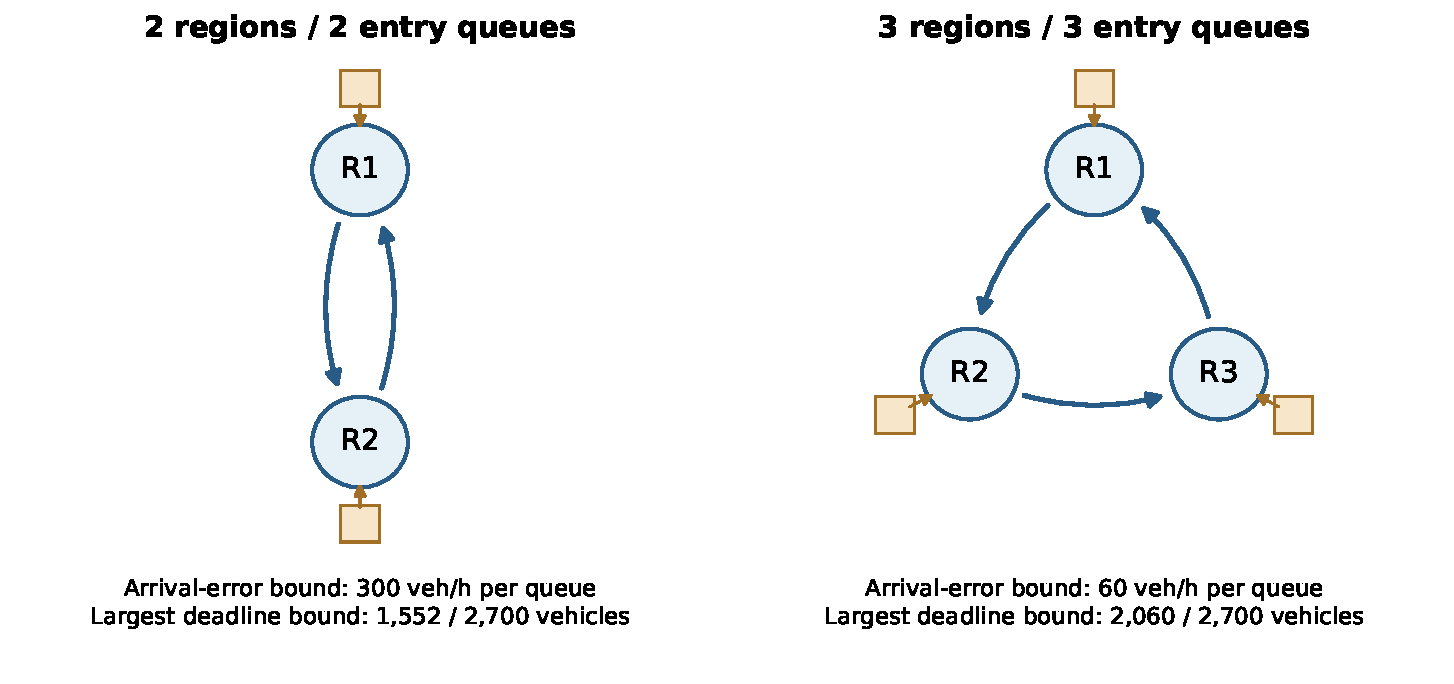
\includegraphics[width=\textwidth]{figures/network_extension_results.pdf}
\caption{Connected-ring certification examples. Circles denote regions,
squares denote exterior entry queues, and arrows denote the directed
interregional transfers and admissions. For a regional initial error
bound of 25 vehicles, the listed arrival-error bounds apply separately
to each queue. The displayed deadline value is the largest certified
regional bound, rounded upward, compared with the common 2700-vehicle
service limit. Routing and admission allocation are fixed as specified
in \appref{app:network-transfer}.}
\label{fig:network-results}
\end{figure}
Successful twelve-state certification checks take 5.20--5.28 seconds for 120 intervals.
The full sweep contains sixteen attempts under the settings in
\appref{app:network-transfer}. These cases illustrate the construction
under fixed routing and allocation assumptions.


